\documentclass[conference]{IEEEtran}

\usepackage{newtxtext}
\usepackage{newtxmath}
\usepackage{amsmath}
\usepackage{balance}
\usepackage{booktabs}
\usepackage{graphicx}
\usepackage{url}
\usepackage{xcolor}
\usepackage[hidelinks]{hyperref}

\hypersetup{
    pdftitle={Temporal-Consensus OCR for Accessible Extraction of Static and Scrolling News Headlines},
    pdfauthor={Sukhraj Singh},
    pdfsubject={Reproducible temporal aggregation for video headline OCR},
    pdfkeywords={optical character recognition, video text, temporal consensus, news ticker}
}

\newcommand{\BenchmarkClips}{50}
\newcommand{\PositiveClips}{40}
\newcommand{\NegativeClips}{10}
\newcommand{\BaselineCER}{12.34\%}
\newcommand{\TemporalCER}{2.10\%}
\newcommand{\BaselineWER}{26.33\%}
\newcommand{\TemporalWER}{9.67\%}
\newcommand{\EnsembleCER}{12.34\%}
\newcommand{\EnsembleWER}{26.83\%}
\newcommand{\BaselineExact}{37.5\%}
\newcommand{\TemporalExact}{70.0\%}
\newcommand{\EnsembleExact}{37.5\%}
\newcommand{\BaselineSuccess}{50.0\%}
\newcommand{\TemporalSuccess}{100.0\%}
\newcommand{\EnsembleSuccess}{50.0\%}
\newcommand{\BaselineFOne}{66.67\%}
\newcommand{\EnsembleFOne}{66.67\%}
\newcommand{\TemporalFOne}{100.00\%}
\newcommand{\SuccessDifference}{50.0}
\newcommand{\BootstrapLow}{35.0}
\newcommand{\BootstrapHigh}{65.0}
\newcommand{\McNemarP}{1.91e-06}
\newcommand{\MedianRuntime}{0.62}


\title{Temporal-Consensus OCR for Accessible Extraction of Static and Scrolling News Headlines}

\author{\IEEEauthorblockN{Sukhraj Singh}
\IEEEauthorblockA{Faculty of Computer Science and Technology\\
Algoma University, Brampton, Ontario, Canada}}

\begin{document}

\maketitle

\begin{abstract}
Text in a television lower-third or scrolling ticker is often absent from the audio transcript,
yet it carries names, locations, and breaking-news updates.  Framewise optical character
recognition (OCR) is inadequate when a moving headline is only partly visible per frame.  This
paper presents a lightweight local pipeline that samples a resolution-independent headline
region; evaluates raw, contrast-equalized, and Otsu-binarized hypotheses; filters recognitions by
confidence and dictionary-free lexical evidence; and aggregates them over time.  Static text is
resolved with a quality-weighted medoid, while scrolling text is reconstructed by fuzzy token
overlap.  A deterministic benchmark generates \BenchmarkClips{} four-second clips: \PositiveClips{}
positives span static and scrolling layouts under four degradation conditions, and
\NegativeClips{} are negative controls.  Against center-frame OCR, temporal consensus reduces
mean character error rate from \BaselineCER{} to \TemporalCER{} and raises sequence success at
normalized similarity 0.80 from \BaselineSuccess{} to \TemporalSuccess{}.  The paired gain is
\SuccessDifference{} percentage points (bootstrap 95\% CI: \BootstrapLow{}--\BootstrapHigh{};
exact McNemar $p=1.91\times10^{-6}$).  These results validate the temporal mechanism, not readiness
for unconstrained broadcasts; real-news, multilingual, and automatic-localization evaluations
remain necessary.
\end{abstract}

\begin{IEEEkeywords}
optical character recognition, video text recognition, temporal consensus, news ticker,
accessibility, reproducible benchmark
\end{IEEEkeywords}

\section{Introduction}

Broadcast video contains two information channels: the audible program and text rendered into
the image.  The latter includes lower-thirds, locations, speaker names, scores, market values,
weather warnings, and continuously scrolling headlines.  Such text is not guaranteed to occur
in closed captions or automatic speech recognition output.  Recovering it is therefore useful
for search, archival, monitoring, and assistive interfaces.

Reading text from video is more difficult than recognizing a scanned page.  Characters may be
small, blurred by motion, distorted by compression, or superimposed on a changing background.
The ICDAR video-text literature identifies illumination change, camera motion, blur, and
real-time constraints as persistent problems \cite{karatzas2013icdar,cheng2021svts}.  More
importantly for a ticker, the desired sequence is not present in any one image.  A single frame
can be recognized perfectly and still be an incomplete answer.

The original course prototype used a fixed pixel crop, Tesseract, a dictionary threshold, and a
set of unique strings.  It was neither resolution independent nor reproducibly evaluated, and
dictionary filtering could reject newsworthy proper nouns.  Its reported confusion matrix could
not be regenerated.  This ground-up revision asks: \emph{How much can lightweight temporal
aggregation improve headline recovery over single-frame OCR when the text region is known?}

The contributions are threefold:
\begin{enumerate}
    \item A CPU-oriented extraction pipeline that separates spatial localization, OCR
    hypotheses, confidence-aware filtering, static consensus, and scrolling-text assembly.
    \item A deterministic video generator and paired evaluation protocol covering two motion
    modes, four controlled degradations, negative controls, ablations, and error-rate metrics.
    \item An open implementation with tests, machine-readable predictions, regenerated result
    tables, and a high-contrast browser report with local text-to-speech controls.
\end{enumerate}

This empirical systems paper contributes a reproducible, interpretable temporal layer rather
than a new OCR neural architecture.

\section{Related Work}

\subsection{OCR and Scene Text}

Tesseract established a widely used open OCR pipeline built around line finding, adaptive
classification, and linguistic processing \cite{smith2007tesseract}.  Modern scene-text systems
couple learned detectors with sequence recognizers.  EAST directly predicts oriented word or
line geometry \cite{zhou2017east}; CRAFT models character regions and affinities
\cite{baek2019craft}; and differentiable binarization learns the thresholding operation within a
segmentation detector \cite{liao2020db}.  PP-OCR emphasizes lightweight deployability
\cite{du2020ppocr}, with later versions revising both detection and recognition components
\cite{li2022ppocrv3}.  The implementation evaluated here uses the small PP-OCRv6 recognition
model distributed by RapidOCR; PP-OCRv6 is currently documented as a preprint rather than a
peer-reviewed result \cite{zhang2026ppocrv6,rapidocr2026}.

The present system assumes a user or upstream component has specified a one-line headline band.
This reduces CPU cost but prevents direct comparison with general scene-text spotters.

\subsection{Video Text and Temporal Evidence}

Nguyen \emph{et al.} used temporal redundancy for video-text recognition on ICDAR-VIDEO and a
YouTube dataset \cite{nguyen2014video}.  Newer benchmarks evaluate localization, tracking, and
complete sequence transcripts \cite{cheng2021svts}; Sequential Transformer models long-term
context jointly for detection and tracking \cite{zhang2024sequential}.  In contrast, this method
aggregates text after ROI selection: it is smaller and inspectable but less general.

\subsection{Preprocessing and Synthetic Evaluation}

Otsu thresholding optimizes gray-level class separation \cite{otsu1979threshold}, while adaptive
histogram equalization improves local contrast \cite{pizer1987adaptive}.  Synthetic data enables
controlled scene-text experiments \cite{gupta2016synthetic}.  Here it is used only for evaluation:
it isolates motion and degradation effects but cannot substitute for a real-broadcast corpus.

\section{Method}

\begin{figure*}[t]
\centering
\setlength{\fboxsep}{7pt}
\fbox{Video frames}
$\longrightarrow$
\fbox{Normalized headline ROI}
$\longrightarrow$
\fbox{Raw / CLAHE / Otsu hypotheses}
$\longrightarrow$
\fbox{PP-OCRv6 line recognition}
$\longrightarrow$
\fbox{Confidence and lexical filter}
$\longrightarrow$
\fbox{Static medoid or ticker assembly}
$\longrightarrow$
\fbox{JSON / accessible HTML}
\caption{Pipeline boundary.  The system recognizes a supplied single-line region rather than
performing unconstrained full-frame text detection.}
\label{fig:pipeline}
\end{figure*}

\subsection{Input, Sampling, and Region of Interest}

Let a video contain frames $F_t$ at source rate $r$.  Frames are sampled at a configurable rate
$r_s$; the experiment uses $r_s=2$ frames/s.  A region
$R=(x,y,w,h)\in[0,1]^4$ is stored in normalized coordinates and converted to pixels for each
frame, eliminating the prototype's resolution-specific crop.  The recognized image hypothesis
for preprocessing variant $v$ is
\begin{equation}
    I_{t,v}=P_v\left(R(F_t)\right), \qquad
    v\in\{\mathrm{raw},\mathrm{CLAHE},\mathrm{Otsu}\}.
\end{equation}
Each crop is enlarged with bicubic interpolation before line recognition.  Because a lower-third
can contain more than one line in practice, this one-line assumption is a deliberate scope limit,
not a general solution to layout analysis.

\subsection{Recognition and Candidate Quality}

For each $I_{t,v}$, the OCR engine returns text $s_{t,v}$ and confidence $c_{t,v}\in[0,1]$.
Unicode is normalized, unsupported symbols are removed, whitespace is collapsed, and comparison
is case insensitive.  Unlike the original dictionary test, proper nouns and acronyms are not
penalized.  Candidate quality is
\begin{equation}
q_{t,v}=0.72c_{t,v}+0.18a_{t,v}+0.10\min(n_{t,v}/8,1),
\end{equation}
where $a_{t,v}$ is the proportion of visible characters that are alphanumeric and $n_{t,v}$ is
the number of word tokens.  A candidate must contain at least three tokens with alphabetic
content and confidence at least 0.30.  This suppresses isolated labels such as ``LIVE'' and
times such as ``8:30 PM'' without requiring an English dictionary.

\subsection{Static Consensus}

Multiple preprocessing outputs from one frame are reduced to the highest-quality candidate.
For a static overlay, the representative string is a quality-weighted medoid.  For candidate
$i$,
\begin{equation}
S_i=q_i+\sum_j q_j\frac{\operatorname{ratio}(s_i,s_j)}{100}
    +\frac{\min(n_i,12)}{20},
\end{equation}
where $\operatorname{ratio}$ is normalized Levenshtein similarity.  Selecting
$\arg\max_i S_i$ rewards agreement across frames while retaining a complete, high-confidence
observation.  It avoids character-level voting, which requires uncertain spatial alignment.

\subsection{Scrolling-Ticker Assembly}

Mode can be set explicitly.  Automatic mode uses near-duplicate support and observed word-count
range: a span of at least two with weak global support indicates a ticker; otherwise repeated
high-similarity observations indicate static text.

Ticker candidates remain in timestamp order.  Near-duplicate adjacent observations are removed.
For two windows $A=(a_1,\ldots,a_m)$ and $B=(b_1,\ldots,b_n)$, the algorithm searches from the
largest possible suffix--prefix overlap downward.  An overlap of length $k$ is accepted when
the mean fuzzy similarity of $(a_{m-k+1},\ldots,a_m)$ and $(b_1,\ldots,b_k)$ is at least 76.
Within the overlap, the longer of two near-matching tokens is retained; this repairs boundary
fragments such as ``OUNCIL''/``COUNCIL'' or ``PL''/``PLAN.''  A character-level overlap of more
than five characters is the fallback.  Competing chains are ranked first by recovered word count
and then by accumulated quality.

Figure~\ref{fig:ticker} shows why temporal assembly is necessary: different frames expose
different, overlapping portions of one sentence.

\begin{figure*}[t]
\centering
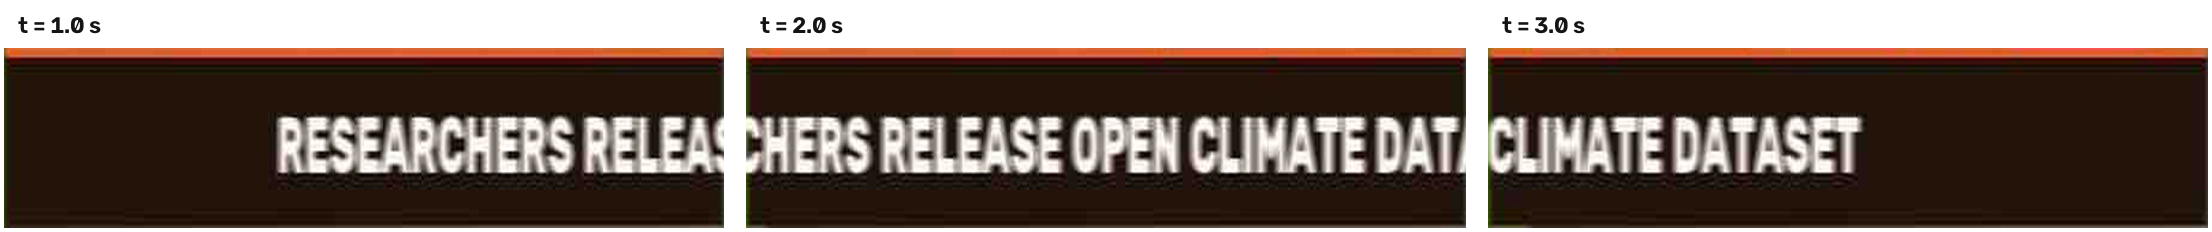
\includegraphics[width=0.98\textwidth]{figures/ticker_sequence.png}
\caption{Three sampled regions from a synthetic ticker under horizontal blur and JPEG
compression.  No displayed crop contains the full reference, ``RESEARCHERS RELEASE OPEN CLIMATE
DATASET,'' but chronological overlaps provide the missing context.}
\label{fig:ticker}
\end{figure*}

\subsection{Accessible Output}

UTF-8 JSON records the transcript, mode, timing, configuration, and retained candidates.  An
optional high-contrast HTML view offers scalable type, keyboard-visible controls, and local
browser speech synthesis.  The visible transcript remains inspectable before playback.

\section{Experimental Design}

\subsection{Controlled Benchmark}

The generator creates \PositiveClips{} positive clips from five neutral, fictional headline
strings crossed with two motion modes and four conditions.  Each MJPG clip is 640$\times$360,
six frames/s, and 24 frames (4 s).  Static text is centered and entirely visible.  Ticker text is
rendered larger than the 600-pixel band and moves right-to-left, so no single crop is guaranteed
to contain the complete sentence.  Conditions are: (1) clean; (2) 30-level low contrast;
(3) Gaussian noise with standard deviation 28; and (4) seven-pixel horizontal blur followed by
JPEG quality 25.  Ten negative clips contain an empty band or a non-headline label.  The random
seed, ground truth, and every rendering parameter are stored in the manifest.

This intentionally small dataset is a mechanism test: motion, visibility, and degradation vary
while the transcript is known exactly.  It does not estimate performance across broadcast
networks, languages, fonts, or graphics packages.

\subsection{Ablations and Metrics}

Three inference conditions use the same sampled video:
\begin{enumerate}
    \item \textbf{Center frame}: raw OCR from the sampled frame nearest the clip midpoint.
    \item \textbf{Center + multiview}: the highest-quality raw, CLAHE, or Otsu hypothesis at
    that frame.
    \item \textbf{Temporal}: automatic static/ticker inference and aggregation over all samples.
\end{enumerate}

For positive clips, character error rate (CER) and word error rate (WER) are Levenshtein distance
divided by reference characters and words, respectively.  Exact-match rate is also reported.
A clip is a sequence-level success when normalized character similarity is at least 0.80.
Negative clips make precision measurable; positive clips determine recall.  The threshold is
declared before comparison and is not an exact-transcription claim.

The success-rate difference is paired by clip.  A seeded 5,000-resample paired bootstrap gives a
95\% percentile interval \cite{efron1979bootstrap}; an exact two-sided McNemar test evaluates the
discordant binary outcomes.  These statistics describe this fixed controlled corpus only.

\subsection{Reproducibility Environment}

Experiments ran on Windows 11 and a 12th-generation Intel Core i5-1235U CPU using Python 3.13.9,
RapidOCR 3.9.2, ONNX Runtime 1.29.0, OpenCV 5.0.0.93, and NumPy 2.5.2.  Inference was CPU-only and
used the packaged PP-OCRv6 small recognizer.  Generated videos are excluded from version control;
one command recreates them and the CSV, JSON, and \LaTeX{} result artifacts.

\section{Results}

\begin{table*}[t]
\caption{Overall controlled-benchmark results.  Lower is better for CER/WER; higher is better
otherwise.  Precision, recall, and F1 use the 0.80 sequence-success rule.}
\label{tab:overall}
\centering
\begin{tabular}{lccccccc}
\toprule
Method & CER $\downarrow$ & WER $\downarrow$ & Exact $\uparrow$ & Success $\uparrow$ & Precision & Recall & F1 \\
\midrule
Center frame & \BaselineCER & \BaselineWER & \BaselineExact & \BaselineSuccess & 100.00\% & 50.00\% & \BaselineFOne \\
Center + multiview & \EnsembleCER & \EnsembleWER & \EnsembleExact & \EnsembleSuccess & 100.00\% & 50.00\% & \EnsembleFOne \\
\textbf{Temporal consensus} & \textbf{\TemporalCER} & \textbf{\TemporalWER} & \textbf{\TemporalExact} & \textbf{\TemporalSuccess} & \textbf{100.00\%} & \textbf{100.00\%} & \textbf{\TemporalFOne} \\
\bottomrule
\end{tabular}
\end{table*}

Table~\ref{tab:overall} shows that preprocessing selection alone does not improve center-frame
OCR: CER is unchanged (12.34\% versus 12.34\%) and WER is slightly worse (26.33\% versus 26.83\%).
Thus the temporal gain cannot be attributed to preprocessing.

Temporal consensus reduces CER by 10.24 percentage points and WER by 16.66 points.  Exact match
rises from 37.5\% to 70.0\%.  All 40 positive clips reach the declared 0.80 similarity threshold,
and all 10 controls are rejected, producing \TemporalFOne{} F1.  The paired success gain is
\SuccessDifference{} points (95\% bootstrap CI \BootstrapLow{}--\BootstrapHigh{}); the exact
McNemar result is $p=1.91\times10^{-6}$.

\begin{table}[t]
\caption{Positive-clip results stratified by motion mode.}
\label{tab:mode}
\centering
\begin{tabular}{llccc}
\toprule
Mode & Method & CER & Exact & Success \\
\midrule
Static & Center frame & 0.87\% & 75\% & 100\% \\
Static & Temporal & \textbf{0.75\%} & \textbf{80\%} & 100\% \\
Ticker & Center frame & 23.80\% & 0\% & 0\% \\
Ticker & Temporal & \textbf{3.45\%} & \textbf{60\%} & \textbf{100\%} \\
\bottomrule
\end{tabular}
\end{table}

Table~\ref{tab:mode} locates the effect.  Static clips are easy for one well-cropped frame, while
all sequence-level gain comes from scrolling clips whose center frame is structurally incomplete.
This supports the mechanism, not a claim that temporal aggregation universally improves OCR.

Across conditions, temporal CER is 1.73\% for clean, 1.97\% for low contrast, 1.73\% for Gaussian
noise, and 2.98\% for blur plus compression.  The blur condition is hardest, but every output
remains above the 0.80 success threshold.  Median end-to-end processing time is
\MedianRuntime{} s per 4-s clip after model initialization, or approximately 0.16$\times$ video
duration on this machine.  This is an offline throughput observation, not an interactive latency
guarantee.

\section{Error Analysis and Discussion}

Twelve temporal outputs are non-exact despite 40/40 threshold successes.  Errors fall into three
classes.  First, blur causes character deletion or duplication, for example ``APPROVES'' becoming
``PPROVES.''  Second, a static crop can lose a word boundary (``TEAMADVANCES'').  Third, fuzzy
ticker reconciliation can preserve a plausible but wrong fragment, such as ``COM CLITY'' for
``COMMUNITY.''  The longest headline is occasionally truncated to ``CHAMPIONSHIP F.''  These
examples explain why 100\% threshold success must not be described as 100\% transcription
accuracy; exact match is 70\% and WER is 9.67\%.

The local pipeline preserves proper nouns, exposes candidates for audit, and separates OCR from
temporal logic.  Its normalized ROI spans resolutions, and ticker assembly recovers information
that no selected frame contains.

The principal limitation is external validity.  The benchmark uses five English strings and one
OpenCV font family on synthetic backgrounds; degradations approximate, rather than reproduce,
broadcast encoders and graphics.  The ROI is supplied, text is horizontal and single-line, and
the recognizer's pretraining data are outside experimental control.  No comparison is made with
cloud OCR, large vision-language models, or end-to-end video text spotters because those systems
solve broader tasks and would require a real annotated dataset.  Confidence is not calibrated,
and the heuristic auto-mode boundary was evaluated on the same controlled design in which it was
developed.  Finally, the accessible interface has not undergone a user study with blind or
low-vision participants.

Errors in names, numbers, or emergency messages can change meaning.  Output should therefore be
presented as machine transcription with visible context and confidence, not an authoritative news
feed.  Future work should use a licensed broadcast corpus, add multi-line detection and tracking,
evaluate multilingual recognition, calibrate uncertainty, and conduct an accessibility study.

\section{Conclusion}

This work replaces an unreproducible framewise prototype with a tested, local, auditable system.
On a controlled 50-clip benchmark, temporal overlap reconstructs scrolling sentences that
center-frame OCR cannot fully observe, reducing CER from \BaselineCER{} to \TemporalCER{} while
exact accuracy remains \TemporalExact{}.  The evidence supports effectiveness for known,
single-line ticker regions under the tested degradations; broader claims require real-world,
multilingual, independently annotated evaluation.

\section*{Acknowledgment}

This manuscript grew from a COSC 4086 course project at Algoma University.  The author thanks
Professor Randy Lin for course guidance.

\balance
\bibliographystyle{IEEEtran}
\bibliography{references}

\end{document}
